\documentclass{article}

\usepackage{fancyhdr}
\usepackage{extramarks}
\usepackage{amsmath}
\usepackage{amsthm}
\usepackage{amsfonts}
\usepackage{tikz}
\usepackage[plain]{algorithm}
\usepackage{algpseudocode}
\usepackage{hyperref}
\usepackage{caption}
\usepackage{subcaption}
\usepackage{minted}

\usetikzlibrary{automata,positioning}

%
% Basic Document Settings
%

% Custom sectioning
\usepackage{sectsty}
\allsectionsfont{\centering \normalfont\scshape}

\captionsetup{justification=centering,
singlelinecheck=false
}
\graphicspath{ {required/} }

\topmargin=-0.45in
\evensidemargin=0in
\oddsidemargin=0in
\textwidth=6.5in
\textheight=9.0in
\headsep=0.25in

\linespread{1.1}

\pagestyle{fancy}
\lhead{\hmwkAuthorName}
\chead{\hmwkClass}
\rhead{\hmwkTitle}
\lfoot{\lastxmark}
\cfoot{\thepage}

\renewcommand\headrulewidth{0.4pt}
\renewcommand\footrulewidth{0.4pt}

\setlength\parindent{0pt}

%
% Create Problem Sections
%

\newcommand{\enterProblemHeader}[1]{
    \nobreak\extramarks{}{Problem \arabic{#1} continued on next page\ldots}\nobreak{}
    \nobreak\extramarks{Problem \arabic{#1} (continued)}{Problem \arabic{#1} continued on next page\ldots}\nobreak{}
}

\newcommand{\exitProblemHeader}[1]{
    \nobreak\extramarks{Problem \arabic{#1} (continued)}{Problem \arabic{#1} continued on next page\ldots}\nobreak{}
    \stepcounter{#1}
    \nobreak\extramarks{Problem \arabic{#1}}{}\nobreak{}
}

\setcounter{secnumdepth}{0}
\newcounter{partCounter}
\newcounter{homeworkProblemCounter}
\setcounter{homeworkProblemCounter}{1}
\nobreak\extramarks{Problem \arabic{homeworkProblemCounter}}{}\nobreak{}

%
% Homework Problem Environment
%
% This environment takes an optional argument. When given, it will adjust the
% problem counter. This is useful for when the problems given for your
% assignment aren't sequential. See the last 3 problems of this template for an
% example.
%
\newenvironment{homeworkProblem}[1][-1]{
    \ifnum#1>0
        \setcounter{homeworkProblemCounter}{#1}
    \fi
    \section{Problem \arabic{homeworkProblemCounter}}
    \setcounter{partCounter}{1}
    \enterProblemHeader{homeworkProblemCounter}
}{
    \exitProblemHeader{homeworkProblemCounter}
}

%
% Homework Details
%   - Title
%   - Due date
%   - Class
%   - Section/Time
%   - Instructor
%   - Author
%

\newcommand{\hmwkTitle}{Homework\ 1}
\newcommand{\hmwkDueDate}{January 23, 2015}
\newcommand{\hmwkClass}{Information Integration on the Web}
\newcommand{\hmwkClassInstructor}{Professor Ambite \& Knoblock}
\newcommand{\hmwkAuthorName}{Tushar Tiwari}

%
% Title Page
%

\title{
    \vspace{2in}
    \textmd{\textbf{\hmwkClass:\ \hmwkTitle}}\\
    \normalsize\vspace{0.1in}\small{Due\ on\ \hmwkDueDate}\\
    \vspace{0.1in}\large{\textit{\hmwkClassInstructor}}
    \vspace{3in}
}

\author{\textbf{\hmwkAuthorName}}
\date{}

\renewcommand{\part}[1]{\textbf{\large Part \Alph{partCounter}}\stepcounter{partCounter}\\}

%
% Various Helper Commands
%

% Useful for algorithms
\newcommand{\alg}[1]{\textsc{\bfseries \footnotesize #1}}

% For derivatives
\newcommand{\deriv}[1]{\frac{\mathrm{d}}{\mathrm{d}x} (#1)}

% For partial derivatives
\newcommand{\pderiv}[2]{\frac{\partial}{\partial #1} (#2)}

% Integral dx
\newcommand{\dx}{\mathrm{d}x}

% Alias for the Solution section header
\newcommand{\solution}{\textbf{\large Solution}}

% Probability commands: Expectation, Variance, Covariance, Bias
\newcommand{\E}{\mathrm{E}}
\newcommand{\Var}{\mathrm{Var}}
\newcommand{\Cov}{\mathrm{Cov}}
\newcommand{\Bias}{\mathrm{Bias}}
\begin{document}

\maketitle

\pagebreak

\begin{flushleft}
\section{Statement of Integrity}
I, Tushar Tiwari, declare that the submitted work is original and adheres to all University policies and acknowledge the consequences that may result from a violation of those rules.
\section{Screenshots}
\begin{figure}[h]
\centering
\fbox{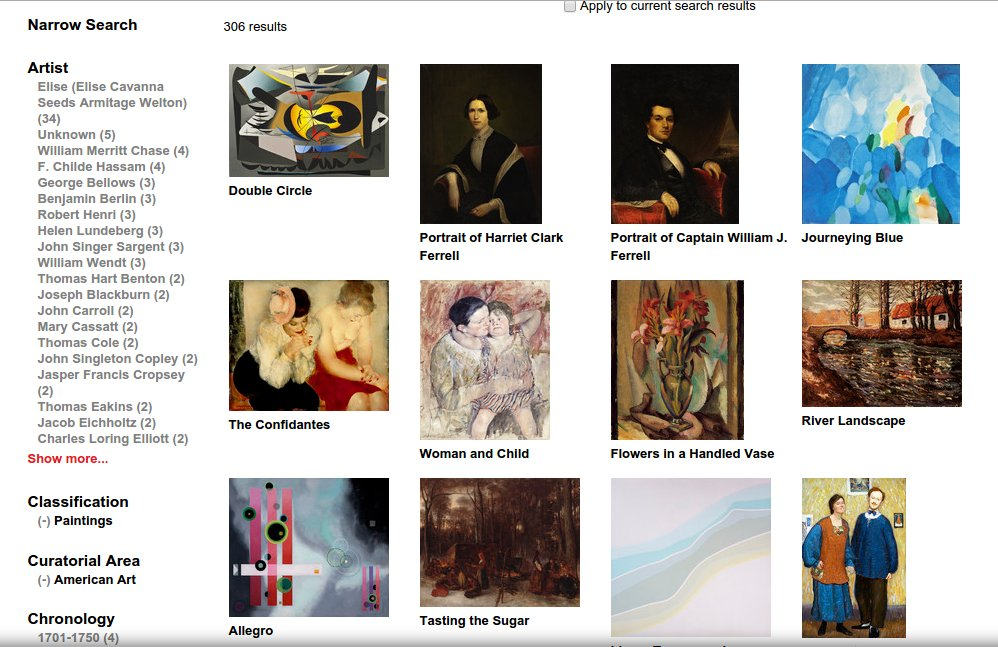
\includegraphics[width=0.6\textwidth]{search}}
\urldef\myurl\url{http://collections.lacma.org/search/site/?page=0&f[0]=bm_field_has_image%3Atrue&f[1]=im_field_curatorial_area%3A32&f[2]=im_field_classification%3A22}
\caption{The search page with the option American Paintings already chosen. \\ This provides us with a custom url that can be exploited to navigate and then extract all paintings. \\ \myurl}
\end{figure}

\begin{figure}[h]
\centering
\begin{subfigure}{0.5\textwidth}
\centering
\fbox{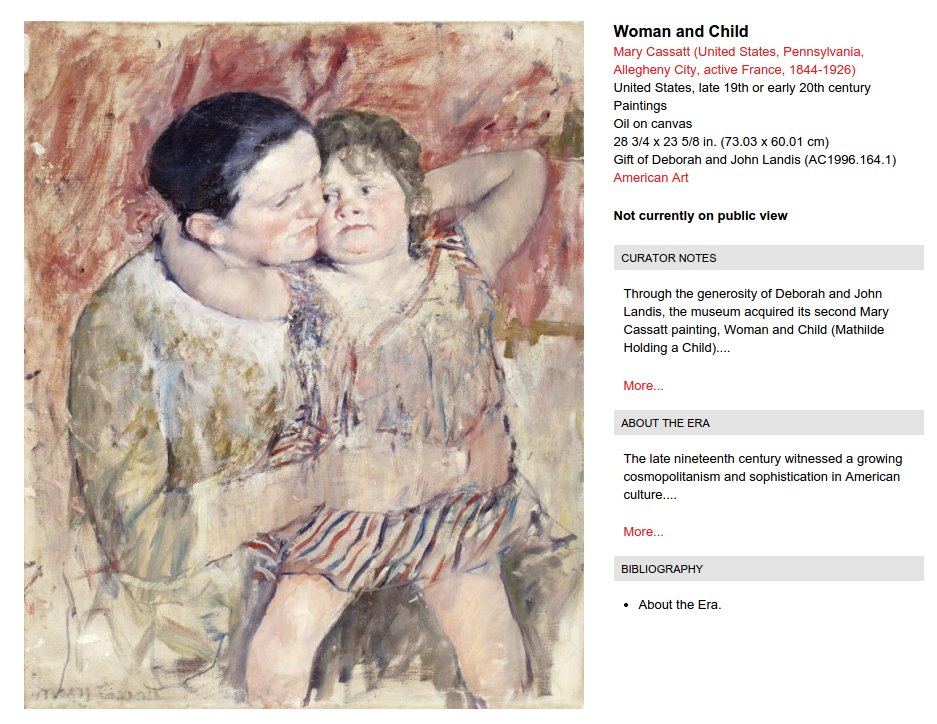
\includegraphics[width=0.95\textwidth]{american-painting}}
\caption{An american painting}
\end{subfigure}%
\begin{subfigure}{0.5\textwidth}
\centering
\fbox{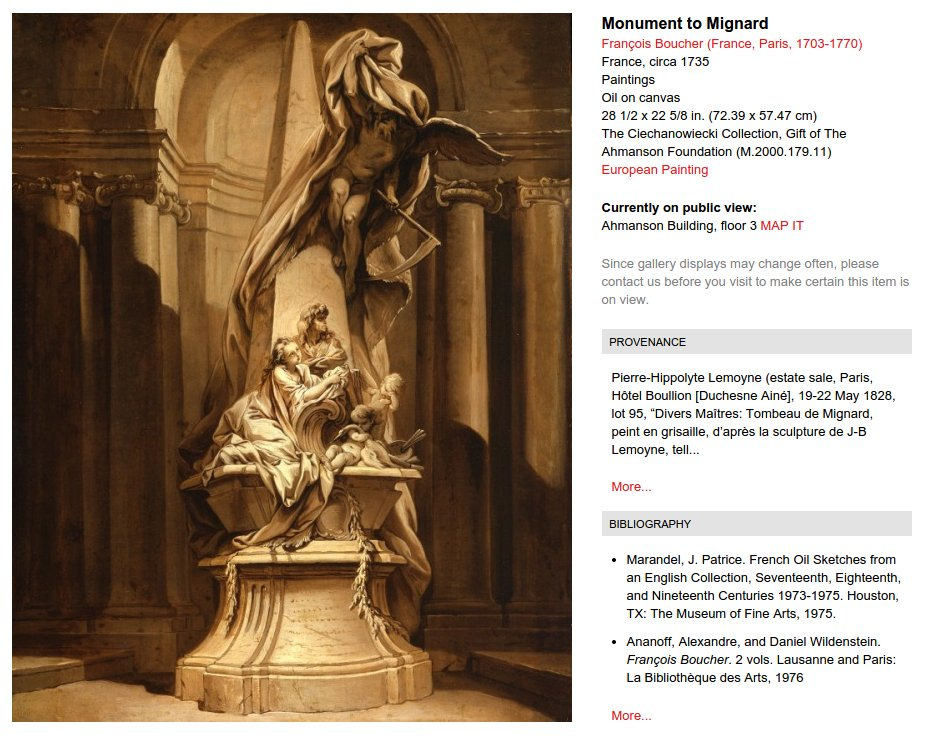
\includegraphics[width=0.95\textwidth]{european-painting}}
\caption{A european painting}
\end{subfigure}
\caption{Examples of the paintings on the website}
\end{figure}
\newpage
\section{Sample Record}
Let's look at a sample painting and the output that it produces. For purposes of demonstration the link to this sample painting is hard-coded into the program so that the output produced is only for the painting in consideration.

\begin{figure}[h]
\centering
\fbox{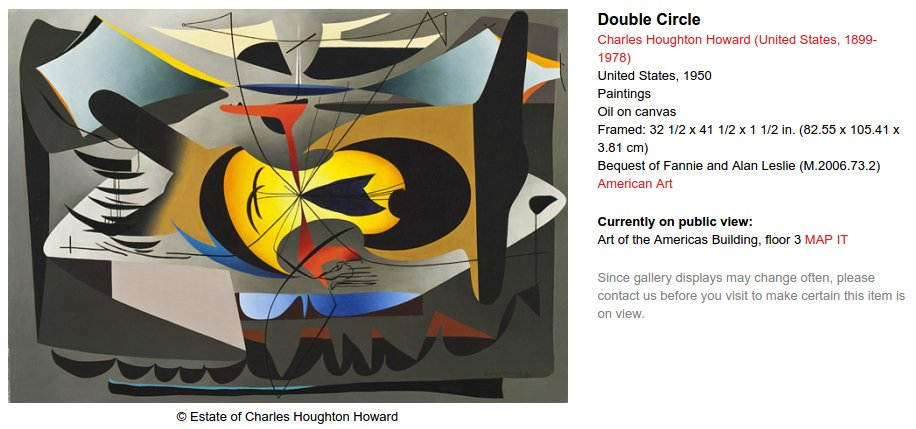
\includegraphics[width=0.98\textwidth]{184481}}
\urldef\myurl\url{http://collections.lacma.org/node/184481}
\caption{The chosen painting found at \myurl.}
\end{figure}

\begin{figure}[h]
\centering
\begin{subfigure}{0.5\textwidth}
\centering
\fbox{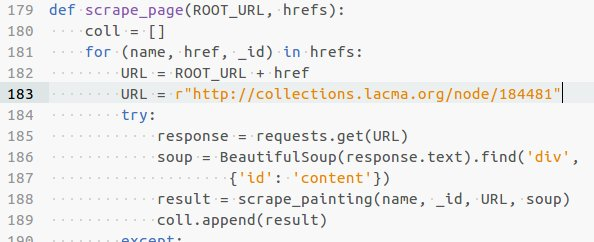
\includegraphics[width=0.95\textwidth]{hardcoding}}
\caption{Hardcoding the url into the code}
\end{subfigure}%
\begin{subfigure}{0.5\textwidth}
\centering
\fbox{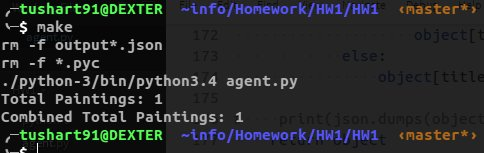
\includegraphics[width=0.95\textwidth]{make}}
\caption{Execution of make command}
\end{subfigure}
\caption{Sample Run}
\end{figure}

\textbf{Note:} 
\begin{itemize}
  \item The url for the painting is hardcoded only for purposes of demonstration. The usual run will automatically extract image urls from the search page.
  \item Not all paintings will have all data fields assosciated with them since the data is unavailable for those paintings. These missing fields have been ignored as they serve no purpose except for increasing the file size which is not desirable.
\end{itemize}
\newpage
\begin{figure}[h]
\centering
\inputminted[frame=single,
               framesep=3mm,
               linenos=true,
               xleftmargin=21pt,
               tabsize=4]{js} {required/output.json}
\caption{Output JSON of sample run}
\end{figure}
\section{Challenges}
\begin{itemize}
  \item Unicode characters are a problem in Python 2 since the default string supports only ascii characters. Due to this certain string operations become very complicated. The problem was oversome by porting the code to Python 3 whose default string supports unicode
  \item Extracting the artist's details required complex regular expressions since all information pertaining to the artist, like name, date of birth, place of birth, was provided in a single string in the html.
\end{itemize}
\newpage

\section{Tools Used}
\subsection{Python with BeautifulSoup}
Python is one of the most easiest to use yet powerful languages out there which works cross-platform. Installing and distributing dependencies is also very easy. Beautiful Soup is a Python library designed for quick turnaround projects like screen-scraping.
It parses anything you give it, and does the tree traversal stuff for you. You can tell it "Find all the links", or "Find all the links of class externalLink", or "Find all the links whose urls match "foo.com", or "Find the table heading that's got bold text, then give me that text.". Some of the features that make it powerful are:
\begin{itemize}
\item Provides a few simple methods and Pythonic idioms for navigating, searching, and modifying a parse tree: a toolkit for dissecting a document and extracting what you need. It doesn't take much code to write an application
\item {Automatically converts incoming documents to Unicode and outgoing documents to UTF-8. You don't have to think about encodings, unless the document doesn't specify an encoding and Beautiful Soup can't detect one. Then you just have to specify the original encoding.}
\item{Sits on top of popular Python parsers like lxml and html5lib, allowing you to try out different parsing strategies or trade speed for flexibility.}
\end{itemize}

\section{Fields not Extracted}
There were no fields that were left untouched. Every field was extracted. But, not all paintings have data for every field. All fields were checked for data. If valid information was present only then it was extracted.

\end{flushleft}
\end{document}